\documentclass[12pt]{article}
\usepackage{amsmath}
\usepackage{amsfonts}
\usepackage{amssymb}
\usepackage[utf8]{inputenc}
\usepackage[T1,T2A]{fontenc}
\usepackage[english, russian]{babel}
\usepackage{graphicx}
\usepackage{float}
\usepackage[left=2cm,right=2cm,top=2cm,bottom=2cm]{geometry}
\usepackage{wrapfig}
\usepackage{pgfplots}
\usepackage{setspace}
\usepackage{indentfirst}
\usepackage{subfigure}
\usepackage{hyperref}
\usepackage{mathrsfs}
\hypersetup{
    colorlinks=true,
    linkcolor=red,
    urlcolor=magenta,
}
\graphicspath{{pictures/}}

\title{ 
    Лабораторная работа 2.2.1 \\
    <<Исследование взаминой диффузии газов>>
}

\author{Комкин Михаил, Б01-303}
\begin{document}
\maketitle
    \paragraph{Цель работы:}1) регистрация зависимости 
    концентрации гелия в воздухе от времени с помощью датчиков 
    теплопроводности при разных начальных давлениях смеси газов; \\
    2) определение коэффициента диффузии по результатам измерений.
    \paragraph{В работе используются:} измерительная установка; форвакуумный
    насос; баллон с газом (гелий); манометр; источник питания; магазин 
    сопротивлений; гальванометр; секундомер.
\section{Теоретическая часть} 
    Диффузией называется самопроизвольное перемешивание молекул, происходящее вследствие их 
    хаотичного теплового движения. При перемешивании молекул разного сорта говорят о 
    взаимной (или концентрационной) диффузии. Для наблюдения взаимной диффузии необходимо 
    равенство давлений во всей системе (в противном случае возникнет гораздо более быстрое 
    макроскопическое течение газа как сплошной среды).\\

    В системе, состоящей из двух компонетов а и b, плотность потока вещества любого 
    компонента в результате взаимной диффузии определяется законом Фика \ref{Fik}:
    \begin{equation}\label{Fik}
        j_{a} = D_{ab}\frac{\partial n_{a}}{\partial x}, \hspace{0.5cm}
        j_{a} = D_{ba}\frac{\partial n_{b}}{\partial x},
    \end{equation}
    где $D_{ab}$ и $D_{ba}$ = $D$ - коэффициент взаимной диффузии компонетов, а $j_{a,b}$ - 
    плотности потока частиц соответствующего сорта\\
    В данной работе исследуется диффузия примеси лёгкого газа (гелия) на фоне воздуха. 
    Концентрация воздуха п, в условиях опыта предполагается значительно большей, чем 
    концентрация примеси пне, и её относительное изменение в результате взаимной диффузии 
    будет незначительным. Поэтому мы будем описывать только диффузию примеси (гелия) на 
    стационарном фоне воздуха и в дальнейшем, если не оговорено особо, под $n$ будем иметь в 
    виду концентрацию примеси $n_{He}$.\\
    Для исследования взаимной диффузии газов и определения коэффициента диффузии используется 
    установка, изображённая на рис. 1. Два сосуда с объёмами $V1$ и $V2$ соединены трубкой длины
    $l$ и сечения $S$. Сосуды заполнены смесью двух газов при одинаковом давлении, но с 
    различной концентрацией компонентов. Вследствие взаимной диффузии концентрации каждого из 
    компонентов в обоих сосудах с течением времени выравниваются.\\
    Рассмотрим процесс выравнивания концентрации. В общем случае концентрация зависит от 
    координат и времени во всей установке. В наших условиях решение задачи упрощается, 
    поскольку объём соединительной трубки мал по сравнению с объёмами сосудов. В связи 
    этим концентрацию газов внутри каждого сосуда можно считать постоянной по всему объёму 
    сосуда, и предположить, что процесс выравнивания концентраций происходит в основном 
    благодаря диффузии в трубке.\\

    Если бы концентрации в сосудах $V_{1}$ и $V_{2}$ поддерживались постоянными 
    и равными $n_{1}$ и $n_2$, то в трубке уствновился бы стационарный поток 
    частиц $J = -DS\frac{\partial n}{\partial x}$, одинаковый в каждом сечении трубки.
    Следовательно $n(x)$ была бы линейной функцией координаты и $dn/dx = \Delta n/l$,
    где $l$ - длина трубки, откуда получаем
    \begin{equation}\label{sootn2}
        J = -DS\frac{n_1 - n_2}{l}
    \end{equation}
    Предположим, что процесс выравнивания концентраций в сосудах происходит
    достаточно медленно, так что все время успевает установится стационарный
    профиль концентраций и в каждый момент времени справедливо соотношение
    \ref{sootn2}. Исходя из этого получим зависимость концентраций в каждом
    сосуде $n_1$ и $n_2$ от времени.\\
    Обозначим через через $\Delta n_1$ и $\Delta n_2$ изменения концентраций
    в объемах $V_1$ и $V_2$ за время $\Delta t$. Тогда $V_1\Delta n_1$ равно 
    изменению количества компонента в объеме $V_1$, а $V_1\Delta n_1$ - 
    изменению количества компонента в объеме $V_2$. Из закона сохранения 
    вещества следует, что $V_1n_1 + V_2n_2 = const$, откуда $V_1 \Delta n_1 = - V_2\Delta n_2$
    Эти изменения происходят вследствие диффузии, поэтому 
    \begin{equation}\label{3}
        V_1\Delta n_1 = -V_2\Delta n_2 = J\Delta t = -DS\frac{n_1 - n_2}{l}\Delta t
    \end{equation}
    Преобразовав это равенство и введя новую переменную $\Delta n = n_1-n_2$,
    затем проинтегрировав, получим:
    \begin{equation}\label{6}
        \Delta n = \Delta n_0 e^{-t/\tau},
    \end{equation}
    $\Delta n_0$ - разность концентраций примеси в начальный момент времени,
    \begin{equation}\label{7}
        \tau = \frac{V_1V_2}{V_1+V_2} \frac{l}{SD}
    \end{equation}
\section{Эксперементальная установка}
\begin{figure}[H]
	\begin{center}
		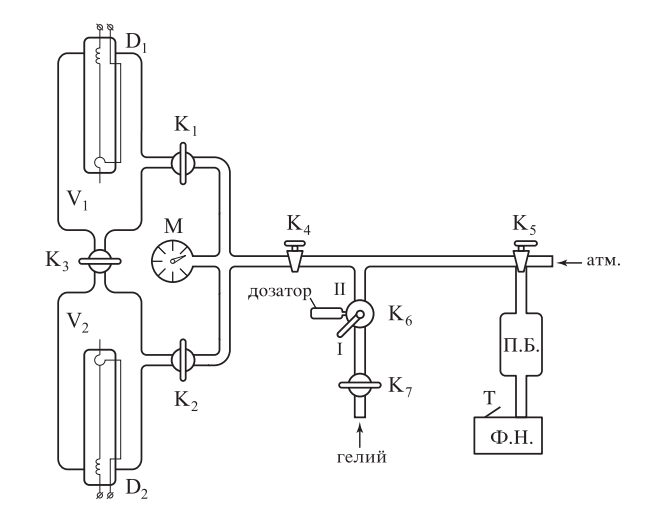
\includegraphics[width = 0.8\textwidth]{установка.png}
		\caption{Схема экспериментальной установки}
		\label{fig:facility}
	\end{center}
\end{figure}
Общий вид конструкции установки приведён на \ref{fig:facility}.\\
Установка состоит из двух сосудов $V_1$ и $V_2$, соединённых краном $K_3$, форвакуумного насоса Ф.Н. с выключателем $Т$, манометра $М$ и
системы напуска гелия, включающей в себя краны $К_6$ и $К_7$. Кран $К_5$ позволяет соединять форвакуумный насос либо с установкой, 
либо с атмосферой. \\
Между форвакуумным насосом и краном $К_5$ вставлен предохранительный баллон П.Б., защищающий кран $К_5$ и установку при неправильной
эксплуатации её от попадания форвакуумного масла из насоса Ф.Н. Сосуды $V_1$ и $V_2$ и порознь и вместе можно соединять как с системой 
запуска гелия, так и с форвакуумным насосом. Для этого служат краны $K_1$, $K_2$, $К_4$ и $K_5$. Манометр М регистрирует давление газа, до 
которого заполняют тот или другой сосуды.\\
Давление гелия в трубопроводе больше атмосферного. Это необходимо для того, чтобы из-за возможных неплотностей в трубопроводе гелий 
оставался бы в нём без примесей воздуха. А система напуска гелия, особенно многоходовой кран $К_6$, как правило, имеет утечки. 
Для сохранения гелия, а также для уменьшения неконтролированного попадания гелия в установку (по протечкам в кране $К_6$) между 
трубопроводом подачи гелия и краном $К_6$ поставлен металлический кран $К_7$. Его открывают только на время непосредственного заполнения 
установки гелием. Все остальное время он закрыт.\\
В силу того, что в сосуд требуется подавать малое давление гелия, между кранами $К_7$ и $К_4$ стоит кран $К_6$, снабженный дозатором. 
Дозатор - это маленький объём, который заполняют до давления гелия в трубопроводе, а затем уже эту порцию гелия с помощью крана 
$К_6$ впускают в установку.\\
Кран $К_4$ обладает повышенной вакуумоплотностью. Как отмечалось выше, кран $К_6$ такой плотностью не обладает. 
Поэтому после заполнения сосудов $V_1$ и $V_2$ рабочей смесью кран $К_4$ надо обязательно закрыть, чтобы в рабочей части 
установки давление в процессе измерений сохранялось постоянным.\\
\section{Ход работы}
    \begin{enumerate}
        \item Включите питание электрической схемы установки рубильником (рис. 2). Откройте краны К1, К2, К3 (рис. 1).
        \item Очистите установку от всех газов, которые в ней есть. Для этого откройте кран К4. Включите форвакуумный насос (Ф.Н.) 
        выключателем Т, находящемся на насосе, и соедините насос с установкой, повернув ручку крана К5 длинным концом рукоятки влево 
        (на установку). Откачайте установку до давления ~0,1 торр,1 что достигается непрерывной работой насоса в течение 3-5 минут. 
        Для прекращения откачки ручку крана К5 поставьте длинным концом вверх. Если при этом выключите и форвакуумный насос, 
        то ручку крана К5 необходимо повернуть вправо, чтобы полость форвакуумного насоса была соединена с атмосферой. 
        В противном случае масло, находящееся в форвакуумном насосе, может быть выдавлено из него и попасть в установку, 
        что недопустимо.
        \item Затем в установку нужно напустить воздух до рабочего давления (вначале Р 40 торр), чтобы сбалансировать мост на 
        рабочем давлении. Для этого (если насос выключен) рукоятку крана К5 повернуть из положения вправо (воздух поступает в насос) 
        в положение влево (воздух из насоса поступает в установку). Эту операцию надо повторить несколько раз, пока не будет 
        достигнуто нужное давление. Если окажется, что воздуха напустили слишком много, излишки его откачать тем же насосом. 
        Сбалансируйте мост. Балансировку моста начинайте при сопротив-
        лении магазина сопротивлений Mr 10° Ом, добиваясь нулевых показаний гальванометра Г вначале с помощью ручки «грубо» 
        (рис. 2), постепенно уменьшая сопротивление магазина до 0, а затем с помощью ручки «точно». Окончательный баланс моста 
        проводите на диапазоне измерений гальванометра 1 мкА. Когда баланс достигнут, переключатели моста установить на максимум. 
        Это необходимо сделать для того, чтобы в процессе последующих действий не сжечь гальванометр. Диапазон измерений 
        самого гальванометра переведите на 10 мкА.
        \item Заполните установку рабочей смесью: в сосуде V2 должен быть воздух, а в сосуде Vi - смесь воздуха, с гелием. 
        Заполнение производится в следующем порядке:
        a) Откачайте установку до ~0,1 торр.
        б) Закройте краны К2 и К3, убедитесь в том, что краны К1 и открыты.
        К4
        b) Заполните объём V1 гелием до давления 0,1 Ррабочее: т. е.4 торр. Давление гелия в трубопроводе немного выше атмосферного 
        и, следовательно, много больше требуемых 4 торр. Поэтому соединять напрямую полость установки с трубопроводом гелия нельзя. 
        Гелием наполняют сначала дозатор (маленький объём), а уже потом (рис. 3) дозатор соединяют с полостью установки. 
        Эту операцию проводят с помощью крана Кб, поворачивая его рукоятку из положения I в положение II и обратно до тех пор, 
        пока не будет достигнуто нужное давление. Если давление гелия оказалось 
        слишком большим, его излишки можно откачать насосом. Гелий можно откачать 
        и весь, а затем вновь заполнить до нужного давления. Такая 
        операция повысит надёжность того, что напущен чистый гелий, а не0
        его смесь с воздухом. После заполнения ёмкости V1 гелием кран К1 
        необходимо закрыть, а из патрубков установки откачать оставшийся 
        гелий до ~0,1 торр.
            в) Откройте кран K2 и с помощью крана K5 заполните объём V3 воздухом до давления 1,5 Ррабочее. После этого закройте кран K1. Это необходимо сделать потому, что его герметичность выше, чем у остальных соединений справа от него, и особенно у крана Кв.
            г) Уравняйте давление в объёмах Vi и V2, открыв кран K1 при уже 
            открытом кране К2 (кран К3 открывать пока нельзя). Не торопитесь 
            закрывать краны К1 и К2 хотя бы потому, что в одном сосуде происходит 
            адиабатическое сжатие, а в другом разрежение. Поэтому температура 
            газов в одном сосуде будет повышаться, а в другом понижаться.
            Необходимо, чтобы исходное состояние было изотермическим. Пока 
            идёт выравнивание давлений и температур, подготовьте измерительную 
            схему к работе. Для этого, постепенно уменьшая величину 
            сопротивления Mr. добейтесь такого состояния, чтобы стрелка 
            гальванометра показывала ~95 делений от всей шкалы. Если и при 
            Mr = 0 отклонение стрелки гальванометра мало, увеличьте 
            чувствительность шкалы гальванометра, переключая последовательно 
            с 10 мкА до 5 мкА или 1 мкА. Если у вас на эту процедуру уходит 
            времени больше, чем 1-2 минуты, то прежде чем продолжать её дальше, 
            закройте краны К1 и К3. Затем закончите работу с гальвано метром.
        \item Приступите к измерениям. Откройте кран К3, включите 
        кундомер и отмечайте, как изменяются показания гальванометра 
        с течением времени. Процесс измерений продолжайте до тех пор, 
        пока разность концентраций (показания гальванометра) не упадёт 
        на 30-50 (при этом должно быть снято не менее 10 точек).
        Продолжайте аналогичные измерения (пп. 3-6) при различных значениях давления.
        \item Внесем полученные данные в таблицу. Здесь ее проводить не будем, так как
        потребуется слишком много места.
    
        \item Убедитесь, что процесс диффузии подчиняется закону (6). 
        С этой целью для каждого из давлений постройте графики, 
        откладывая по оси абсцисс время, а по оси ординат - логарифм 
        от показаний гальванометра. Графики должны иметь вид прямых 
        линий. По угловым коэффициентам экспериментальных прямых и 
        известным параметрам установки рассчитайте коэффициенты взаимной 
        диффузии при выбранных вами давлениях.
        \begin{figure} [H]
            \caption{График зависимости $V(t)$}
            \centering 
            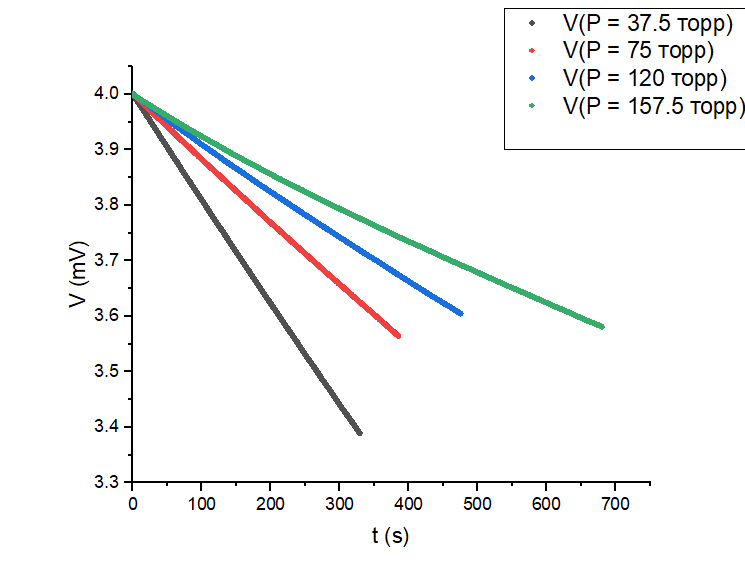
\includegraphics[scale=0.7]{image.png} 
        \end{figure}
        \begin{table}[H]
            \centering
            \begin{tabular}{|c|c|c|c|c|c|}
                \hline
                $ P $, торр & $ \sigma_P $, торр & $ B \cdot 10^{-3} $, с$ ^{-1} $ & $ \sigma_{B} \cdot 10^{-3} $, с$ ^{-1} $ & $ \tau $, с & $ \sigma_\tau $, с \\ \hline
                37.5 & 1,9 & -18.62 & 0.01 & 53.7 & 0,1 \\ \hline
                75 & 1,9 & -11.34 & 0.01 & 88.2 & 0,1 \\ \hline
                120 & 1,9 & -8.29 & 0,09 & 120.3 & 0,2 \\ \hline
                157.5 & 1,9 & -6.05 & 0,02 & 165.3 & 0,4 \\ \hline
            \end{tabular}
            \caption{Аппроксимация зависимостей}
            \label{tab:approx}
        \end{table}
        \item Рассчитаем коэффициент диффузии по формуле \[D = -\frac{VL}{2\tau S}\]
        Для этого запишем геометрические параметры установки. $V_1 = (800 \pm 5) \text{см}^3$,
        $V_2 = (800 \pm 5) \text{см}^3$, $L/S = (15.0 \pm 0.1) \frac{1}{\text{см}}$
        При этом погрешность
        \[ \sigma_\tau = \tau \cdot \frac{\sigma_{B}}{|B|}. \]
        \begin{table}[H]
            \centering
            \begin{tabular}{|c|c|c|c|}
                \hline
                $ P $, торр &$ \sigma_P $, торр & $ D $, $ \frac{\text{см}^2}{\text{с}} $ & $ \sigma_D $, $ \frac{\text{см}^2}{\text{с}} $ \\ \hline
                26.6 & 1.35 & 34.9 & 0.03 \\ \hline
                13.3 & 0.34 & 21.3 & 0.08 \\ \hline
                8.3 & 0.13 & 15.6 & 0.14 \\ \hline
                6.4 & 0.07 & 11.3 & 0.54 \\ \hline
            \end{tabular}
            \caption{Результаты вычислений $D$}
            \label{tab:Dres}
        \end{table}
        \begin{figure} [H]
            \caption{Зависимость коэффициента диффузии от 
            давления в координатах $D, 1/Р$}
            \centering 
            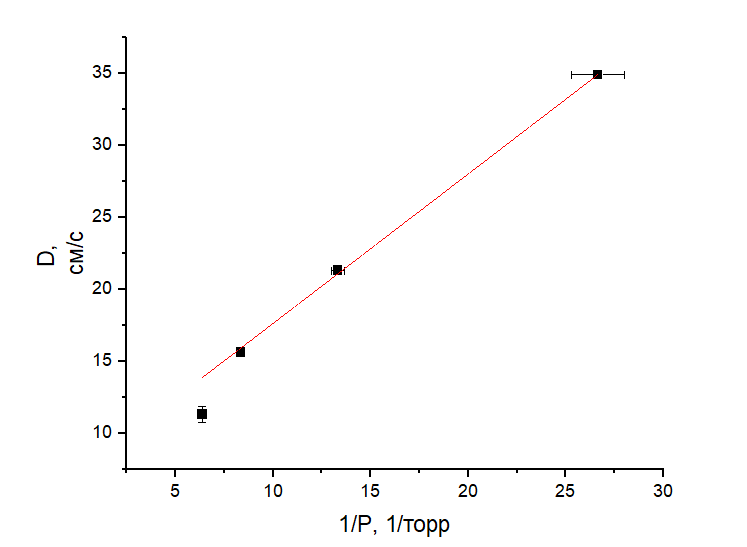
\includegraphics[scale=0.8]{p).png} 
        \end{figure}

        \item Построим график зависимости коэффициента диффузии от 
        давления в координатах $D, 1/Р$. Рассчитаем величину коэффициента диффузии при атмосферном 
        давлении.
        \[ k = (437.36 \pm 21.01)\frac{\text{см}^2}{\text{с*торр}}\]
        и 
        \[ \boxed {D_{\text{атм}} = (0.55\pm 0.03)\frac{\text{см}^2}{\text{с}}}\]
        
        \item Посчитаем длину свободного пробега гелия в данных условиях:
        \begin{equation}
        \sigma_{\lambda_{He}} = \lambda_{He}\cdot \frac{\sigma_D}{D}
        \end{equation}
        \begin{equation}
        \lambda_{He} = \frac{3D}{\bar{\upsilon}} = \frac{3D}{\sqrt{\frac{8RT}{\pi \mu}}}= ( 1.2 \pm 0.12 ) \cdot 10^{-7} \text{м}
        \end{equation}
        
        Из выражения для длины свободного пробега можно найти эффективное сечение столкновений атомов гелия с молекулами воздуха:
        \begin{equation}
        \sigma_\sigma = \sigma \sqrt{(\frac{\sigma_p}{p})^2+(\frac{\sigma_\lambda}{\lambda})^2}
        \end{equation}
        \begin{equation}
        \sigma = \frac{1}{n_0\lambda} = \frac{kT}{p\lambda}= ( 3.4 \pm 0.3 ) \cdot 10^{-19} \text{м}^2
        \end{equation}
        Основоной вклад в данную погрешность дает неточность измерения давления.

    \end{enumerate}
    \section{Вывод}
        Получено значение коэффициента взаимной диффузии гелия и воздуха при разных пропорциях, видна идентичность полученных результатов при разных пропорциях газов и при сравнении с табличными значениями.
    \end{document}